\chapter{Stereoscopic Video}
\markright{Stereoscopic Video}
\label{stereo_video}
\phantomsection
%\addcontentsline{toc}{chapter}{Stereoscopic Video}

In a wide variety of image processing applications, explicit depth information is required in
addition to general image informations, such as intensities, color, densities.\\
Examples of such applications are found in 3D vision (robot vision, photogrammetry, remote sensing systems), in medical imaging (computer tomography,
magnetic resonance imaging, microsurgery), in remote handling of objects (random bin picking), in space exploration (mobile robotics navigation) or 3D movies and videogames.\\
In each of these cases, depth information is essential for accurate image analysis or for enhancing the
realism.\\
In remote sensing the terrain's elevation needs to be accurately determined for map production, in remote handling an operator needs to have precise knowledge of the threedimensional organization of the area to avoid collisions and misplacements.\\
\begin{figure}[h!]
\centering
\begin{subfigure}[]{0.5\textwidth}
		\centering
        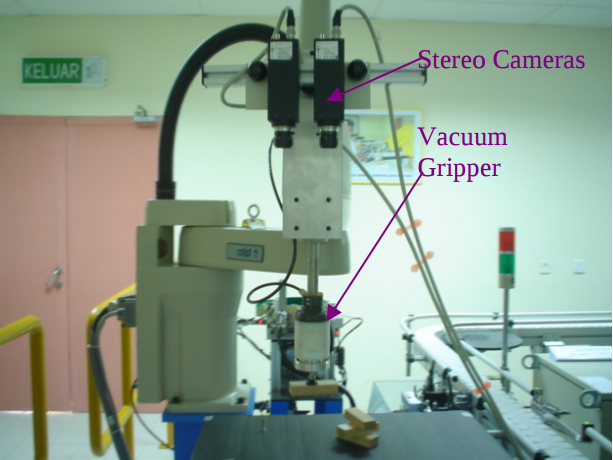
\includegraphics[width=0.7\textwidth]{./img/bin_pick.png}
                \caption{\scriptsize{In bin picking applications stereo vision helps to reconstruct the 3D environment and detect the part of the object to be robotically picked}}
\end{subfigure}% 
~ \quad
\begin{subfigure}[]{0.5\textwidth}
	\centering
	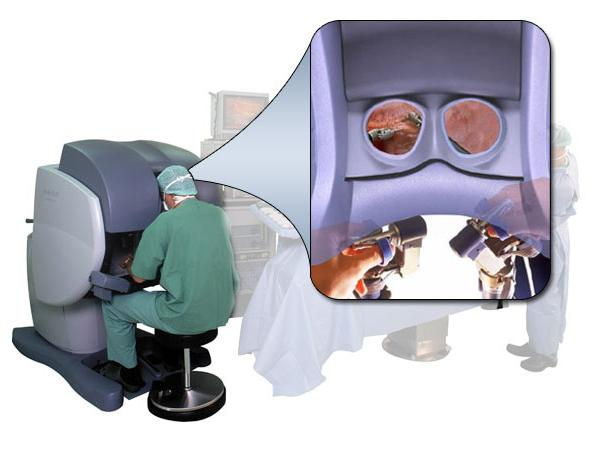
\includegraphics[width=0.7\textwidth]{./img/da_vinci.jpg}
          \caption{\scriptsize{Surgical robot \textit{Da vinci} is provided with a stereoscopic camera that allows a tridimensional view of the operative filed.}}
\end{subfigure} 
\caption{\small{Stereoscopy in medical and industrial field}}
\end{figure}

\begin{figure}[h!]
\centering
\begin{subfigure}[]{0.5\textwidth}
		\centering
        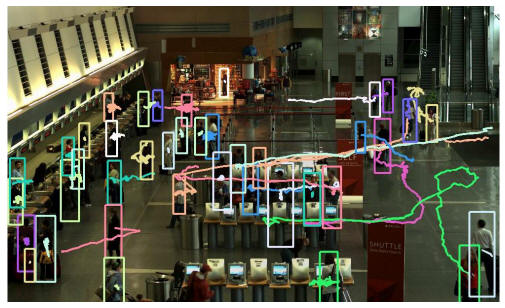
\includegraphics[width=0.7\textwidth]{./img/tracking.jpg}
                \caption{\scriptsize{In people tracking application stereo vision improves segmentation thanks to depth information and it's less sensible to light changes.}}
\end{subfigure}% 
~ \quad
\begin{subfigure}[]{0.5\textwidth}
		\centering
        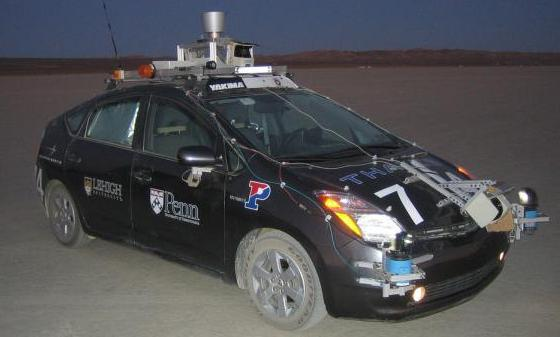
\includegraphics[width=0.7\textwidth]{./img/little_ben.jpg}
                \caption{\scriptsize{In mobile robotics navigation stereo vision has became the first choice technology because it provids a lot of quality data for low costs.}}
\end{subfigure} 
\caption{\small{Stereoscopy application's fields}}
\end{figure}
Depth in real world scenes can be explicitly measured by a number of range sensing devices such as by laser range sensors, by structured light or by ultrasound.
However it's usually undesirable to have separate systems for acquiring the intensity and the depth
information because of the relative low resolution of the range sensing devices and because it's not an easy task to fuse information from different type of sensors; for these reasons and for a non-negligible economic factor stereoscopic vision has becoming the technology of choice in these type of applications.
\begin{figure}[h!]
\centering
\begin{subfigure}[]{0.4\textwidth}
		\centering
        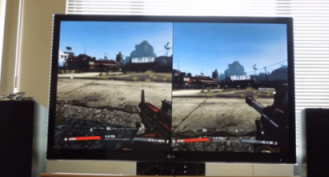
\includegraphics[width=0.7\textwidth]{./img/games1.png}
                \caption{\scriptsize{Stereo video frames, left and right.\newline}}
\end{subfigure}
\begin{subfigure}[]{0.4\textwidth}
		\centering
        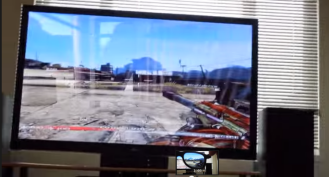
\includegraphics[width=0.7\textwidth]{./img/games2.png}
                \caption{\scriptsize{Overlap of the two frames.}}
\end{subfigure} 
\begin{subfigure}[]{0.4\textwidth}
		\centering
        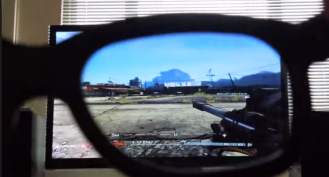
\includegraphics[width=0.7\textwidth]{./img/games3.png}
                \caption{\scriptsize{3D view with specific glasses}}
\end{subfigure}%
\begin{subfigure}[]{0.4\textwidth}
		\centering
        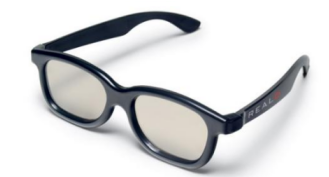
\includegraphics[width=0.7\textwidth]{./img/games4.png}
                \caption{\scriptsize{Polarized glasses for 3D view}}
\end{subfigure} 
\caption{\small{Stereoscopy in 3D video games}}
\end{figure}

\section{Stereo vision}
In image processing stereo vision is the process of extracting 3D information from multiple 2D views of a scene. \\
The 3D information can be obtained from a pair of images, also known as a stereo pair, by estimating the relative depth of points in the scene.\\
From the anatomic point of view, the human brain calculates the depth in a visual scene mainly by
processing the information brought by the images seen by the left and the right eyes. These left and right images are slightly different because the eyes have biologically different emplacements.\\
Consequently, the straightforward way of achieving stereoscopic digital imaging is to emulate the
Human Visual System (HSV) by setting-up (under controlled geometric positions), two traditional 2D
cameras.\\
\begin{figure}[h]
\centering
\begin{subfigure}[b]{0.35\textwidth}
        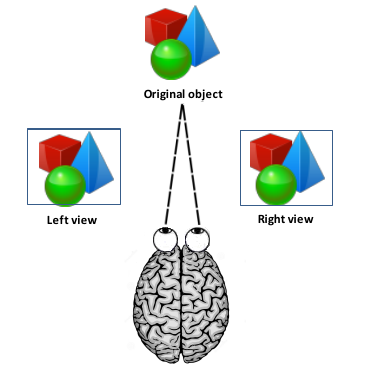
\includegraphics[width=\textwidth]{./img/hvs.png}
         \caption{\scriptsize{Binocular human visual system}}
         \label{fig:hvs}
\end{subfigure}
\begin{subfigure}[b]{0.35\textwidth}
        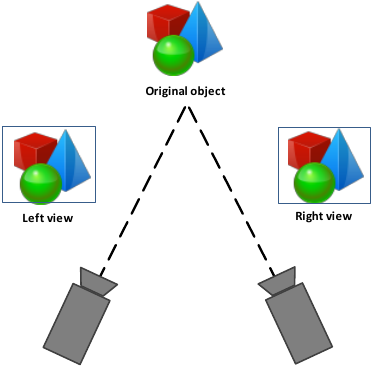
\includegraphics[width=\textwidth]{./img/stereo.png}
        \caption{\scriptsize{Stereoscopic system}}
        \label{fig:stereo}
\end{subfigure} 
\caption{\small{Binocular human vision vs. stereoscopic content acquisition.}}
\end{figure}

\subsection{Acquisition of stereoscopic images}\label{sec:acquisition-of-stereoscopic-images}

In order to be able to perceive depth using recorded images, a stereoscopic camera is required,
which consists of two cameras that capture two different, horizontally shifted perspective
viewpoints; with two (or more) cameras we can infer depth, by means of triangulation, if we are able to find corresponding points in the two images (Figure \ref{fig:corr}).\\
\begin{figure}[h!]
\centering
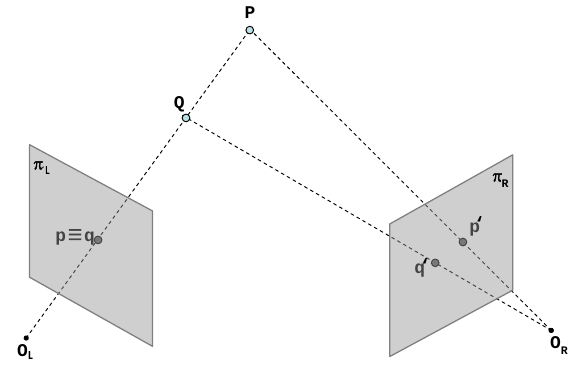
\includegraphics[width=0.6\textwidth]{./img/correspondance.png}
\caption{\small{Triangulation: with two cameras the depth of }}
\label{fig:corr}
\end{figure}
 The camera setup should be geometrically
calibrated such that the two cameras capture the same part of the real world scene.\\
Calibration of a stereo camera system involves the estimation of the intrinsic and extrinsic parameters of the model: intrinsic parameters embody the characteristics of the optical system and its geometric relationship with the image sensor, extrinsic parameters relate the location and orientation of the second camera with respect to the first one in the 3D space (Figure \ref{fig:rt}).\\
\begin{figure}[h!]
\centering
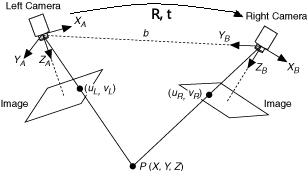
\includegraphics[width=0.6\textwidth]{./img/stereo_system.png}
\caption{\small{Stereo camera model}}
\label{fig:rt}
\end{figure}
These parameters can be used to rectify a stereo pair of images to make them appear as the two image planes are parallel (Figure \ref{fig:rect_stereo}); once the images are rectified, epipolar geometry it's used to find corresponding points and compute the disparity map.
\begin{figure}[h!]
\centering
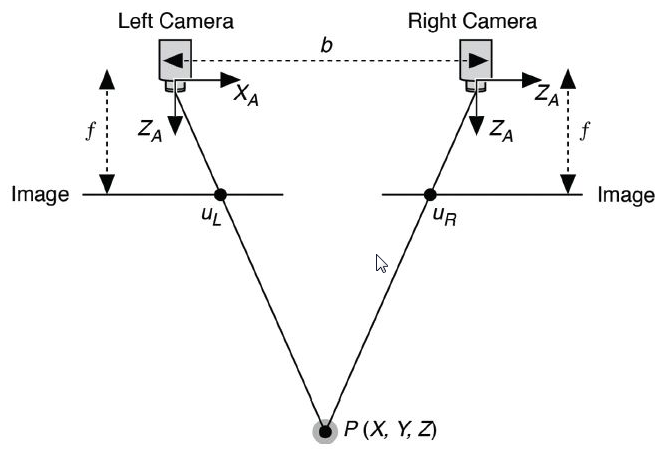
\includegraphics[width=0.6\textwidth]{./img/rect_stereo.png}
\caption{\small{Rectified stereo cameras}}
\label{fig:rect_stereo}
\end{figure}
\begin{figure}[h!]
\centering
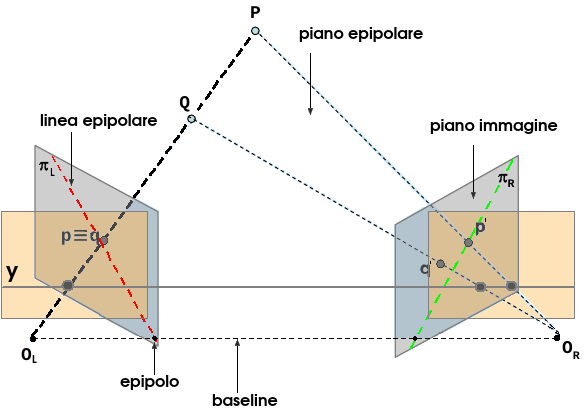
\includegraphics[width=0.6\textwidth]{./img/standard.png}
\caption{\small{Rectified images: corresponding points (p, p'), projection of the same 3D point (P) are constrained on the same image horizontal line, the epipolar line}}
\label{fig:std}
\end{figure}

\newpage
\subsection{Disparity map computation}

With the stereo rig in standard form and by considering similar triangles in Figure \ref{fig:depth} (PO$_{L}$O$_{R}$ and Ppp'): 
$$
\frac{b}{Z} = \frac{(b+x_{L}) - x_{R}}{Z-f} 
$$ 
so
$$
Z = \frac{b \cdot f}{x_{L} - x_{R}} = \frac{b \cdot f}{d}
$$ 

where $ d = x_{L} - x_{R} $ it's called \textit{disparity}.\\
\begin{figure}[h!]
\centering
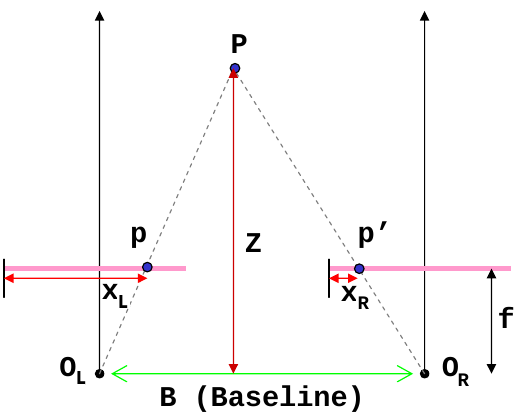
\includegraphics[width=0.6\textwidth]{./img/depth.png}
\caption{\small{Geometry of standard form}}
\label{fig:depth}
\end{figure}
Disparity is, therefore, the difference between the $x$ coordinates of two corresponding points and it is usually encoded with greyscale image (Figure \ref{fig:disparity}), where points closer to the cameras are brighter and correspond to a higher disparity.\\
\begin{figure}[h!]
\centering
\begin{subfigure}[]{0.4\textwidth}
\centering
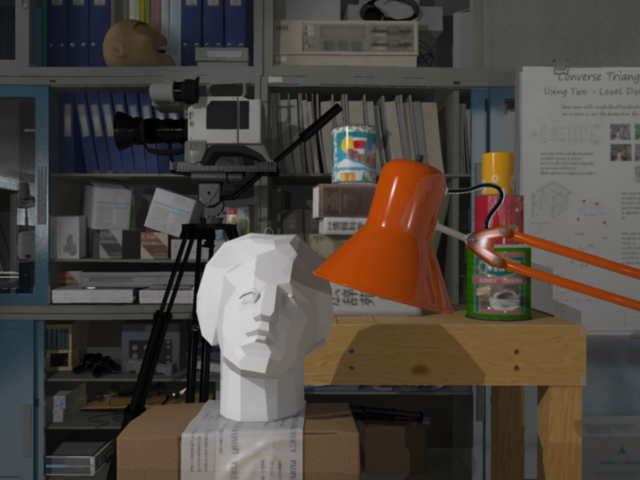
\includegraphics[width=0.7\textwidth]{./img/left.png}
\caption{\scriptsize{Left image}}
\end{subfigure}% 
~ %add desired spacing between images, e. g. ~, \quad, \qquad, \hfill etc.$  $
  %(or a blank line to force the subfigure onto a new line)
\begin{subfigure}[]{0.4\textwidth}
\centering
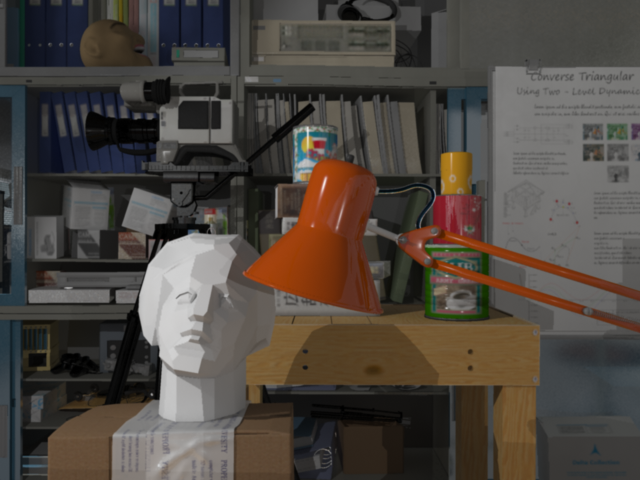
\includegraphics[width=0.7\textwidth]{./img/right.png}
\caption{\scriptsize{Right image}}
\end{subfigure} 
~\quad
\begin{subfigure}[]{0.4\textwidth}
\centering
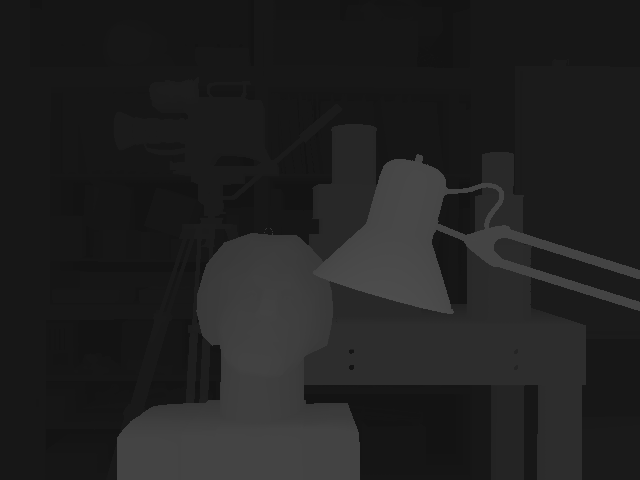
\includegraphics[width=0.7\textwidth]{./img/disparity.png}
\caption{\scriptsize{Disparity map}}
\label{fig:disparity}
\end{subfigure}%
\caption{\small{Stereo pair and disparity map}}
\end{figure}
In order to compute the disparity map is necessary to find corresponding points; stereo correspondance is though a challenging task that has to manage with perspective distortions, uniform and ambiguous regions, repetitive patterns, occlusions and discontinuities(Figure \ref{fig:occl}).\\
\begin{figure}[h!]
\centering
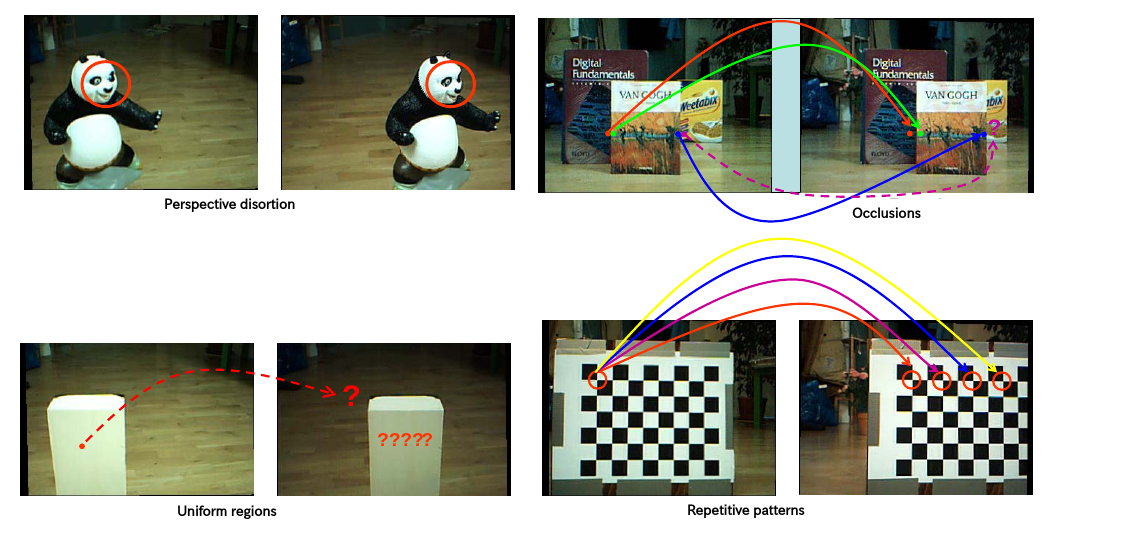
\includegraphics[width=0.6\textwidth]{./img/occl.png}
\caption{\small{Stereo matching general problems}}
\label{fig:occl}
\end{figure}
In general, stereo matching algorithms can be categorized into two major classes:
\begin{itemize}
\item[-] local methods 
\item[-] global methods.
\end{itemize}
Local stereo algorithms estimate the correspondence using a local support region or a window. Local algorithms generally rely on an approximation of the smoothness constraint assuming that all pixels within the matching region have the same disparity. However, this assumption is not valid for highly curved surfaces or around disparity discontinuities.\\
A naive approach consists of comparing each  pixel or window in the left image with every pixel or window on the same epipolar line in right image and picking position with minimum match cost (e.g., SSD, SAD, normalized correlation).\\ 
\begin{figure}[h!]
\centering
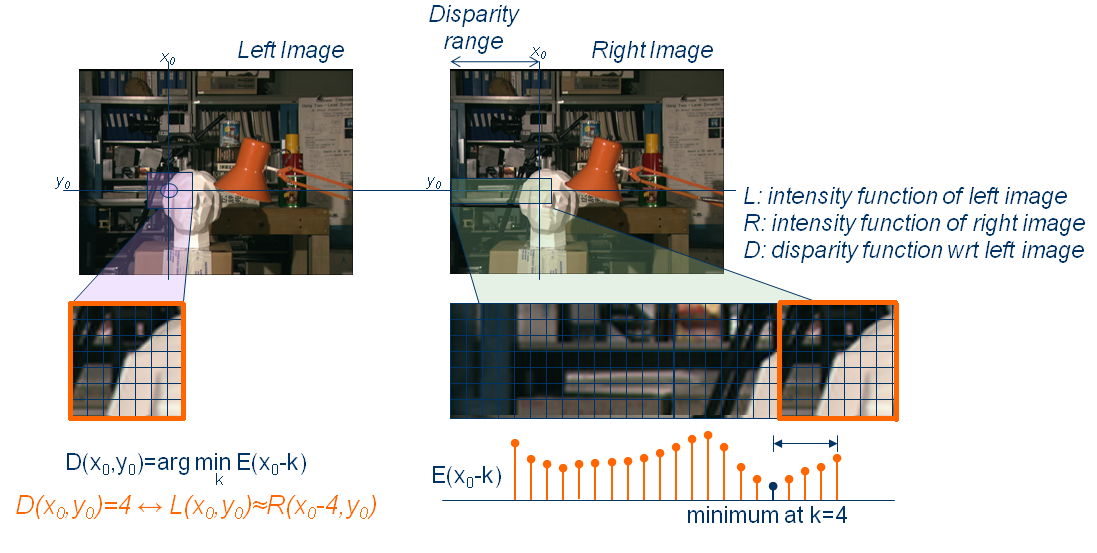
\includegraphics[width=0.7\textwidth]{./img/local.png}
\caption{\small{Local stereo matching, window based}}
\label{fig:local}
\end{figure}
Global stereo methods consider stereo matching as a labeling problem where the pixels of the reference image are nodes and the estimated disparities are labels. An energy functional embeds the matching assumptions by its data, smoothness, and occlusion terms and propagates them along the scan line or through the whole image. The labeling problem is solved by energy functional minimization, using dynamic programming, graph cuts, or belief propagation.\\
Even if this class of algorithms is significantly slow, the results, especially when textures and discontinuities are present, are much accurate.\\
\newline
In this thesis the Kolmogorov and Zabih's Graph Cuts Stereo Matching Algorithm, \cite{KZ}, has been used, because there were no time constraints requirements and the quality of the computed disparities has been considered satisfying with regard to the ground trouth.\\
\begin{figure}[h!]
\centering
\begin{subfigure}[]{0.4\textwidth}
\centering
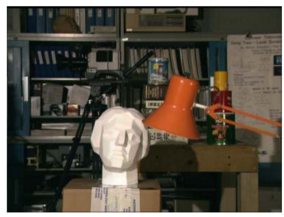
\includegraphics[width=0.7\textwidth]{./img/gf1.png}
\caption{\scriptsize{Left image}}
\end{subfigure}% 
~ %add desired spacing between images, e. g. ~, \quad, \qquad, \hfill etc.$  $
  %(or a blank line to force the subfigure onto a new line)
\begin{subfigure}[]{0.4\textwidth}
\centering
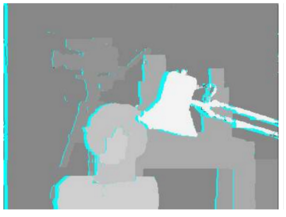
\includegraphics[width=0.7\textwidth]{./img/gf2.png}
\caption{\scriptsize{Graph cuts' disparity map}}
\end{subfigure} 
~\quad
\begin{subfigure}[]{0.4\textwidth}
\centering
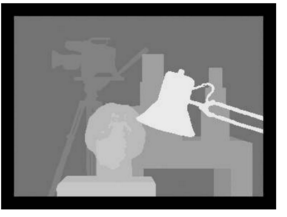
\includegraphics[width=0.7\textwidth]{./img/gf3.png}
\caption{\scriptsize{Ground truth disparity map}}
\label{disparity}
\end{subfigure}%
\caption{\small{Results of the Kolmogorov and Zabih's graph cuts algorithm on the Tsukuba pair}}
\end{figure}
\newline
\section{3D capturing devices}
For stereoscopic shooting, two synchronized cameras must be used. The distance between the center of the lenses of the two cameras is called the interaxial, and the cameras' convergence, is called the angulation. These two parameters can be modified according to the expected content peculiarities.\\
\begin{figure}[h!]
\centering
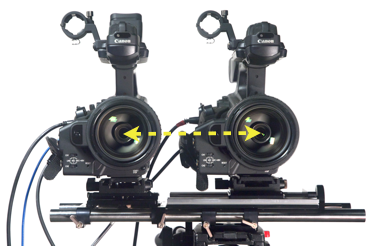
\includegraphics[width=0.3\textwidth]{./img/interaxial-separation.png}
\caption{\small{Interaxial separation between lenses}}
\label{fig:interaxial}
\end{figure}
The two cameras must be correctly aligned, identically calibrated (i.e. brightness, color, etc...) and perfectly synchronized (frame-rate and scan-wise).\\
To hold and align the cameras, a stereo-rig is used; the rigs can be of two main types:\\
\begin{itemize}
\item[-] the side-by-side rig, where the cameras are placed side by side (Figure \ref{fig:sbs}). This kind of 3D-rig is mostly useful for large landscape shots since it allows large interaxials; however, it doesn't allow small interaxials because of the physical size of the cameras;
\begin{figure}[h!]
\centering
\begin{subfigure}[]{0.4\textwidth}
\centering
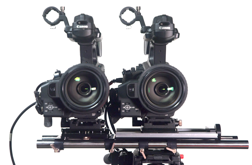
\includegraphics[width=0.7\textwidth]{./img/syderig.png}
\caption{\scriptsize{Syde-by-syde rig}}
\label{fig:sbs}
\end{subfigure}% 
~ %add desired spacing between images, e. g. ~, \quad, \qquad, \hfill etc.$  $
  %(or a blank line to force the subfigure onto a new line)
\begin{subfigure}[]{0.25\textwidth}
\centering
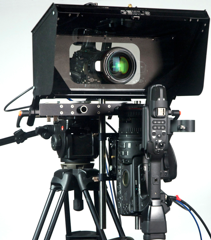
\includegraphics[width=0.7\textwidth]{./img/mirrorrig.png}
\caption{\scriptsize{Beamsplitter rig}}
\label{fig:beam}
\end{subfigure} 
~\quad
\begin{subfigure}[]{0.4\textwidth}
\centering
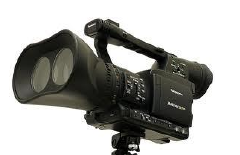
\includegraphics[width=0.7\textwidth]{./img/monorig.png}
\caption{\scriptsize{Monoblock camera}}
\label{fig:mono}
\end{subfigure}%
\caption{\small{Professional technologies for 3D TV }}
\end{figure}
\item[-] the beamsplitter rig (Figure \ref{fig:beam}), where one camera films through a semi-transparent mirror, and the other films the reflection in the mirror. These rigs allow small and medium interaxials, useful for most shots, but not the very large interaxials (because the equipment would be too large and heavy).\\
\end{itemize}
Monoblock cameras have been designed as well, where the two cameras are presented in a fixed block
and are perfectly aligned, which avoids cameras desynchronization (Figure \ref{fig:mono}).\\
A second category of 3D shooting devices is presented in Figure \ref{fig:mobile}. These electronic devices are less expensive and are targeting the user-created stereoscopic picture/movie distribution.\\
\begin{figure}[h!]
\centering
\begin{subfigure}[]{0.4\textwidth}
\centering
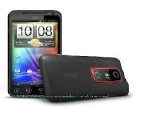
\includegraphics[width=0.7\textwidth]{./img/devices1.png}
\caption{\scriptsize{Mobile phones}}
\end{subfigure}% 
~ %add desired spacing between images, e. g. ~, \quad, \qquad, \hfill etc.$  $
  %(or a blank line to force the subfigure onto a new line)
\begin{subfigure}[]{0.25\textwidth}
\centering
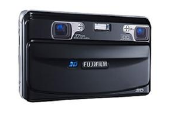
\includegraphics[width=0.7\textwidth]{./img/devices2.png}
\caption{\scriptsize{Digital cameras}}
\end{subfigure} 
\begin{subfigure}[]{0.4\textwidth}
\centering
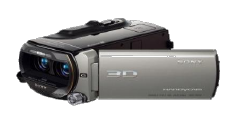
\includegraphics[width=0.7\textwidth]{./img/devices3.png}
\caption{\scriptsize{Camcorders}}
\end{subfigure}%
\caption{\small{Digital personal stereo vision systems}}\label{fig:mobile}
\end{figure}
An other important category of 3D image capture devices it's the one employed in the robotics and automation field. They are usually impressively precise, cost-efficient and fast.
\begin{figure}[h!]
\centering
\begin{subfigure}[]{0.4\textwidth}
\centering
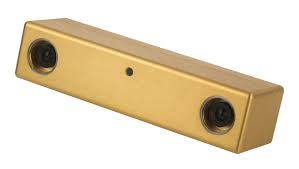
\includegraphics[width=0.7\textwidth]{./img/bumble.jpg}
\caption{\scriptsize{The Bumblebee series from Point Grey}}
\end{subfigure}
\begin{subfigure}[]{0.3\textwidth}
\centering
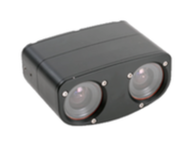
\includegraphics[width=0.7\textwidth]{./img/stereodevices.png}
\caption{\scriptsize{Human wearable stereo device}}
\end{subfigure}
\caption{\small{Industrial and robotic stereo cameras}}
\end{figure}
\section{3D video displays}
The basic technique of stereo displays is to present offset images that are displayed separately to the left and right eye. Both of these 2D offset images are then combined in the brain to give the perception of 3D depth.\\
For stereoscopic 3D displays the viewer needs to wear special glasses which separate the views of the stereoscopic image for the left and the right eye. These 3D glasses can be active or passive.\\
On the one hand, active glasses are controlled by a timing signal that allows to alternatively darken one
eye glass, and then the other, in synchronization with the refresh rate of the screen. Hence presenting
the image intended for the left eye while blocking the right eye's view, then presenting the right-eye
image while blocking the left eye, and repeating the process at a high speed which gives the perception
of a single 3D image. This technology generally uses liquid crystal shutter glasses(Figure \ref{fig:glass1}).\\
On the other hand, passive glasses are polarization-based systems and contain a pair of opposite polarizing filters; each of them passes light with similar polarization and blocks the opposite polarized light (Figure \ref{fig:glass2}). Passive 3D TV screens sport a filter with alternating horizontal and vertical stripes, separated by a black, picture-blanking bars. When used with glasses which have corresponding polarising lenses, alternate frames are presented to each eye to create a 3D image.\\
The color anaglyph-based systems are a particular case of the passive glasses and use a color filter for
each eye, typically red and cyan, Figure \ref{fig:glass3} . The anaglyph 3D image contains two images encoded using the same color filter, thus ensuring that each image reaches only one eye.
\begin{figure}[h!]
\centering
\label{fig:glass}
\begin{subfigure}[]{0.4\textwidth}
\centering
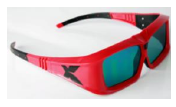
\includegraphics[width=0.7\textwidth]{./img/glass1.png}
\caption{\scriptsize{LCD shutter glasses}}
\label{fig:glass1}
\end{subfigure}% 
~ %add desired spacing between images, e. g. ~, \quad, \qquad, \hfill etc.$  $
  %(or a blank line to force the subfigure onto a new line)
\begin{subfigure}[]{0.4\textwidth}
\centering
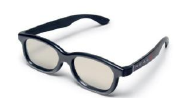
\includegraphics[width=0.7\textwidth]{./img/glass2.png}
\caption{\scriptsize{Polarized glasses}}
\label{fig:glass2}
\end{subfigure} 
\begin{subfigure}[]{0.4\textwidth}
\centering
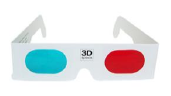
\includegraphics[width=0.7\textwidth]{./img/glass3.png}
\caption{\scriptsize{Anaglyph glasses}}
\label{fig:glass3}
\end{subfigure}%
\caption{\small{Passive and active glasses for 3D viewer technologies}}
\end{figure}
